% !TEX program = xelatex
% 2026 年高教社杯全国大学生数学建模竞赛 A 题
% 补充节：rho–C 直线的斜率截距比作为"是否考虑收缩"的统一判据
%
% 定位：作为问题四之后的收口讨论，与问题二、三的"固定半径"假设形成呼应。
% 并入整篇论文时，把本文件 \section 及其后全部内容取到
% \section{结果文件说明} 之前即可；插图需复制到 论文/figs/。

\documentclass[12pt,a4paper,fontset=none]{ctexart}

\usepackage{xeCJK}
\setmainfont{Times New Roman}
\setsansfont{Arial}
\setCJKmainfont{Songti SC}
\setCJKsansfont{Heiti SC}

\usepackage{amsmath,amssymb,bm}
\usepackage{booktabs}
\usepackage{multirow}
\usepackage{array}
\usepackage{geometry}
\usepackage{caption}
\usepackage{graphicx}

\geometry{left=2.7cm,right=2.7cm,top=2.6cm,bottom=2.6cm}
\captionsetup{font=small,labelsep=quad}
\linespread{1.32}
\allowdisplaybreaks

\begin{document}

\section{关于``是否考虑收缩''的再讨论：斜率截距比给出的统一判据}

问题一至问题三在固定半径 $R=2$\,cm 下求解（假设 A4、B3），问题四改用
附件 2 的实测 $R(t)$ 并在贴体坐标下求解。这两个选择在正文中是分别作出的，
本节说明它们其实由同一个量决定：\textbf{附录密度经验式 $\rho=a+bC$ 的
斜率与截距之比 $r=b/a$}。由 $r$ 可以直接判定该不该考虑收缩、忽略收缩会
带来多大误差，从而使问题二、三的固定半径假设与问题四的动边界模型互相呼应，
而不是两套彼此不相干的简化。

\subsection{判据：收缩只由一个无量纲数决定}

由干基含水率的定义可得恒等式 $\rho=\rho_d(1+C)$，其中
$\rho_d=m_d/V$ 为以湿物料体积为基准的表观干物质密度（第 6 节）。
以 $1$\,kg 干物质为基准写出比体积 $v=V/m_d$，并把经验式 $\rho=a+bC$ 代入，
即得
\begin{equation}
  v(C)=\frac{V}{m_d}=\frac{1+C}{a+bC}
        =\frac{1}{a}\cdot\frac{1+C}{1+rC},
  \qquad r\equiv\frac{b}{a}.
  \label{eq:r-v}
\end{equation}
式 \eqref{eq:r-v} 把一个含两个系数的经验式化归为"一个尺度 $+$ 一个形状"：
$a=\rho(0)$ 只提供尺度（绝干表观密度），而\textbf{收缩规律的形状完全由
无量纲的 $r$ 决定}。于是有
\begin{equation}
  r=1 \iff v(C)\equiv\frac{1}{a}\ \text{为常数}
       \iff \rho_d\ \text{为常数} \iff \text{干燥全程体积不变（无收缩）},
  \label{eq:r-criterion}
\end{equation}
而 $r<1$ 对应"失水后体积收缩"，$r$ 越小收缩越强。也就是说，
\textbf{"要不要考虑收缩"并不是一个需要另行论证的物理判断，而是可以直接
从题面系数读出的判据}：只需看斜率是否等于截距。

题面两条经验式分别给出
\begin{equation}
  r_3=\frac{128}{650}=0.197,\qquad r_4=\frac{90}{760}=0.118 .
  \label{eq:r-values}
\end{equation}
两者都明显小于 $1$，即\textbf{题目给出的两条密度式本身就隐含了收缩}，
且附录 4 的隐含收缩强于附录 3。反过来，若强行要求"斜率等于截距"，
$C_0=2.55$ 处将得到 $\rho=a(1+C_0)=2307.5$\,kg/m$^3$（附录 3），
超过水（$1000$）与干物质真密度（约 $1400$）所能构成的任何混合物密度，
物理上不可能——真正不能成立的是"无收缩"这一要求本身。

\begin{figure}[htb]
  \centering
  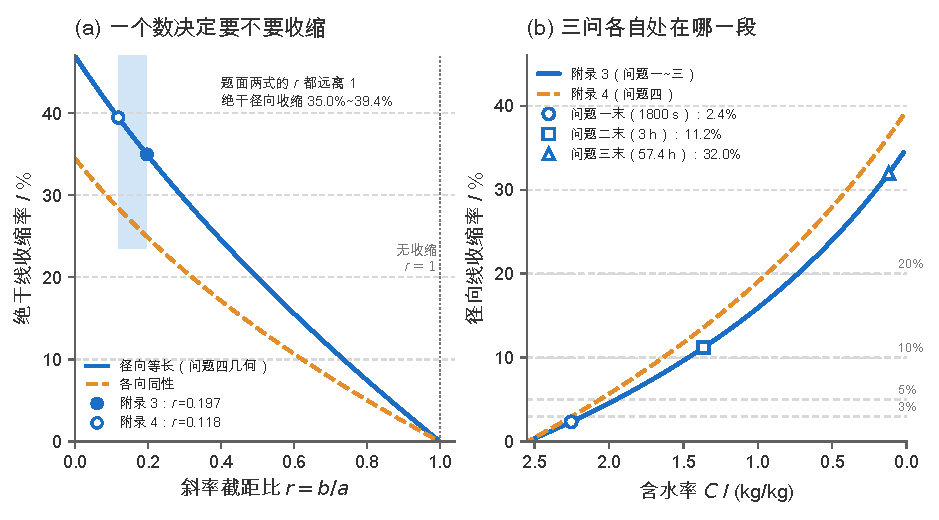
\includegraphics[width=\textwidth]{figs/t01_r_criterion.pdf}
  \caption{(a) 由式 \eqref{eq:r-v} 给出的判据曲线：横轴为斜率截距比
    $r=b/a$，纵轴为该经验式隐含的\textbf{绝干线收缩率} $1-R(0)/R_0$
    （径向等长口径，见 \S\ref{sec:r-geom}）。$r=1$ 时恒为零（无收缩），
    $r$ 越小收缩越强；题面两式的 $r=0.197$、$0.118$ 都远离 $1$，
    对应绝干径向收缩 $35.0\%$ 与 $39.4\%$（阴影带标出题面两式的位置）。
    (b) 同一含水率下的径向线收缩率，三条灰虚线为 $3\%$、$5\%$、$10\%$
    门槛；$\circ$、$\square$、$\triangle$ 分别是问题一、二、三结束时刻
    的体积平均状态，可见三问依次落在"可忽略—已不可忽略—必须考虑"
    三个区间。全部数值由 \texttt{compute\_shrinkage.py} 从结果文件生成。}
  \label{fig:r-crit}
\end{figure}

\subsection{由 $r$ 反推的收缩总量，及其与附件 2 的互证}
\label{sec:r-geom}

由式 \eqref{eq:r-v} 可直接写出任意两个含水率之间的体积比
\begin{equation}
  \frac{V(C)}{V(C_0)}
  =\frac{(1+C)\,(1+rC_0)}{(1+C_0)\,(1+rC)},
  \label{eq:r-vratio}
\end{equation}
其中 $C_0=2.55$\,kg/kg 为初始含水率。若把经验式外推到绝干（$C=0$），则
\begin{equation}
  \frac{V(0)}{V(C_0)}=\frac{1+rC_0}{1+C_0}.
  \label{eq:r-dry}
\end{equation}

式 \eqref{eq:r-dry} 只用到 $r$，因此它给出的是"该经验式隐含的收缩总量"。
由于问题四的几何是\textbf{长度不变、只缩半径}（附件 2 只给半径），
体积比与半径比的关系为 $V/V_0=(R/R_0)^2$，故
\begin{equation}
  \frac{R(0)}{R_0}=\sqrt{\frac{1+rC_0}{1+C_0}} .
  \label{eq:r-radius}
\end{equation}
把式 \eqref{eq:r-values} 代入，得附录 3 的绝干半径为 $1.301$\,cm、
附录 4 为 $1.211$\,cm；而附件 2 记录的实测终半径为 $1.198$\,cm。
\textbf{附录 4 的预测与实测只差 $1.1\%$，附录 3 则偏 $+8.6\%$}。
换成线性收缩模型的收缩系数 $\beta$ 表述：由 $r$ 反演得
$\beta_4=0.891$，由附件 2 的实测半径比反标定得 $\beta=0.922$，两者相差
$3.4\%$。

这一步的意义在于：题目为问题四同时提供了附件 2 的实测 $R(t)$ 与附录 4 的
$\rho(C)$，二者表面上互不相干，但\textbf{它们对"干燥全程能缩到多小"
给出的答案是一致的}。因此问题四把附录 4 的物性配附件 2 的几何并非随意
搭配，而是题面数据自身互相印证的结果。主要数值汇总于表 \ref{tab:r-crit}。

\begin{table}[htb]
  \centering
  \caption{斜率截距比判据与收缩量的汇总
    （附录 3：$\rho=650+128C$；附录 4：$\rho=760+90C$；
    $C_0=2.55$、$\rho_w^0=1000$\,kg/m$^3$）}
  \label{tab:r-crit}
  \small
  \setlength{\tabcolsep}{5pt}
  \begin{tabular}{lccc}
    \toprule
    项目 & 附录 3 & 附录 4 & 附件 2 实测 \\
    \midrule
    截距 $a=\rho(0)$ / (kg/m$^3$) & 650 & 760 & --- \\
    斜率 $b$ / (kg/m$^3$)         & 128 & 90  & --- \\
    斜率截距比 $r=b/a$            & 0.197 & 0.118 & --- \\
    绝干体积比 $V(0)/V(C_0)$      & 0.423 & 0.367 & 0.359 \\
    绝干半径 $R(0)$ / cm          & 1.301 & \textbf{1.211} & \textbf{1.198} \\
    收缩系数 $\beta$（端点反演）  & 0.822 & 0.891 & 0.922 \\
    $b$ 的物理容许带（$\beta\in[0,1]$）
      & $[85.6,\,650]$ & $[62.1,\,760]$ & --- \\
    \bottomrule
  \end{tabular}
\end{table}

\textbf{一个必须说明的边界}：$r$ 只决定收缩的\textbf{总量律}，给不出
\textbf{时间律}。把问题四求得的场按体积加权平均含水率 $\bar C$ 折算成
比体积，与由 $\rho(C)$ 反推的比体积在同一 $\bar C$ 下比较（表 \ref{tab:r-path}），
可见附件 2 的实测收缩在时间上\textbf{高度前置}——$22$\,h 内基本完成，
而 $\rho$ 律要求收缩与 $\bar C$ 同步下降。两者在总量上一致，在路径上
相差 $10.6\%\sim22.4\%$。这正是本文问题四直接采用附件 2 的实测 $R(t)$、
而不自行用 $\rho(C)$ 反演一个收缩律的原因：半径以平方进入特征扩散时间，
烘干时长对"什么时刻收缩到多少"是敏感的；而 $r$ 的作用是判定"要不要收缩"
并给出收缩量的量级，不是替代实测几何。

\begin{table}[htbp]
  \centering
  \caption{收缩的"总量一致、路径不同"：同一平均含水率下，附件 2 实测比
    体积与由附录 4（$r_4=0.118$）反推的比体积之比}
  \label{tab:r-path}
  \small
  \begin{tabular}{cccccc}
    \toprule
    时刻 $t$ / h      & 5.0 & 10.0 & 20.0 & 50.0 \\
    \midrule
    半径 $R$ / cm      & 1.424 & 1.273 & 1.210 & 1.200 \\
    体积平均 $\bar C$ / (kg/kg) & 0.959 & 0.510 & 0.221 & 0.112 \\
    比体积相对偏差      & $-21.4\%$ & $-22.4\%$ & $-16.1\%$ & $-10.6\%$ \\
    \bottomrule
  \end{tabular}
\end{table}

需要说明口径：本节统一采用与问题四一致的\textbf{径向等长}口径
（长度 $L=25$\,cm 不变、只缩半径）。若改用各向同性口径（半径与长度按
同一比例缩），相同的体积比给出的线收缩比会小约三分之一——如附录 3 的
绝干线收缩将由 $35.0\%$ 变为 $24.9\%$。两种口径描述的是同一体积变化的
不同几何分配，文中只取一种以避免自相矛盾，本文取与问题四模型一致的前者。

\subsection{三问呼应：忽略收缩在各自的时间窗内是多大的近似}

由式 \eqref{eq:r-vratio} 可以反过来把"忽略收缩"的误差量化成一张门槛表：
给定允许的线收缩比，求出对应的含水率（表 \ref{tab:r-thr}）。以附录 3 为例，
线收缩达到 $3\%$、$10\%$、$20\%$ 分别出现在 $C\approx2.18$、$1.47$、$0.73$。

\begin{table}[htbp]
  \centering
  \caption{线收缩达到给定比例时的含水率 $C$（径向等长口径）}
  \label{tab:r-thr}
  \small
  \begin{tabular}{lcccc}
    \toprule
    线收缩达到 & $3\%$ & $5\%$ & $10\%$ & $20\%$ \\
    \midrule
    附录 3 对应 $C$ & 2.177 & 1.953 & 1.467 & 0.730 \\
    附录 4 对应 $C$ & 2.249 & 2.062 & 1.637 & 0.939 \\
    \bottomrule
  \end{tabular}
\end{table}

把问题一、二、三各自结束时刻的水分浓度场按体积加权平均，再代入
式 \eqref{eq:r-vratio}，即得表 \ref{tab:r-echo}。

\begin{table}[htbp]
  \centering
  \caption{三个问题的报数点对应的隐含径向线收缩（体积平均口径）}
  \label{tab:r-echo}
  \small
  \begin{tabular}{lcccc}
    \toprule
    问题 & 时刻 & 体积平均 $\bar C$ / (kg/kg)
      & 附录 3 线收缩 & 附录 4 线收缩 \\
    \midrule
    问题一（预热平衡）   & 1800\,s   & 2.253 & $2.4\%$  & $2.9\%$ \\
    问题二（恒温干燥初） & 3\,h      & 1.364 & $11.2\%$ & $13.6\%$ \\
    问题三（烘干全程）   & 57.42\,h  & 0.120 & $32.0\%$ & $36.4\%$ \\
    \bottomrule
  \end{tabular}
\end{table}

表 \ref{tab:r-echo} 与图 \ref{fig:r-crit}(b) 一并读，可以看清三问为何作
不同的收缩假设。

\textbf{问题一}结束时整体线收缩只有 $2.4\%$，且集中在最外侧薄层——
忽略收缩是一个误差不足 $3\%$ 的近似，可以直接采用（第 6 节原先只给出"$C\ge2.0$ 时线收缩不足 $3\%$"的定性判断，此处给出了由实测场
积分得到的确切数字）。

\textbf{问题二}的 $3$\,h 时间窗结束时体积平均线收缩已达 $11.2\%$，
说明到这一步"忽略收缩"已经不再是微小量，而是\textbf{按题目分工显式声明的
简化}（假设 B3）：问题二的目标是给出 $3$\,h 内的温度与浓度场，保持固定
几何使问题一至三共用同一套离散格式与同一个求解器，便于三者比较；收缩的
完整影响则由问题四承担。

\textbf{问题三}的判据在 $57.42$\,h 才达成，此时体积平均线收缩已达
$32.0\%$，是三者中唯一"必须考虑"的量级。这正是题目要求问题四单独考察
尺寸变化的原因——若在问题三中沿用固定半径，几何误差将达三成。

可见"是否考虑收缩"并不是一个是非题，而是\textbf{取决于所考察的时间窗内
含水率降到多低}的定量选择；而这条界线由斜率截距比 $r$ 唯一确定。

\subsection{本节结论}

\begin{enumerate}
  \item \textbf{判据}：由 $\rho=a+bC$ 定义的斜率截距比 $r=b/a$ 是收缩的
        唯一控制参数，$r=1$ 当且仅当无收缩。题面两式给出
        $r_3=0.197$、$r_4=0.118$，都远离 $1$——\textbf{考虑收缩是题面
        数据自身要求的，不需要额外的物理假设}；反之，"斜率等于截距"
        会在 $C_0$ 处给出 $2307.5$\,kg/m$^3$，物理上不可能。
  \item \textbf{总量互证}：由 $r$ 反推的绝干半径（附录 4：$1.211$\,cm）
        与附件 2 的实测终半径（$1.198$\,cm）相差 $1.1\%$，说明问题四所配的
        两组数据在收缩总量上互相印证；附录 3 的 $1.301$\,cm 则偏 $+8.6\%$。
  \item \textbf{误差分级}：线收缩 $3\%$、$10\%$、$20\%$ 分别出现在
        $C\approx2.18$、$1.47$、$0.73$（附录 3）。问题一结束时整体仅
        $2.4\%$、问题二结束时 $11.2\%$、问题三结束 $32.0\%$，
        这解释了为什么问题一至三可以采用固定半径、而问题四必须引入动边界，
        也把"忽略收缩"从一句定性假设变成了带数字说明的近似。
  \item \textbf{边界}：$r$ 只给出收缩的\textbf{总量律}，给不出\textbf{时间律}。
        附件 2 的实测收缩在时间上高度前置，同一含水率下其比体积比 $\rho$ 律
        低 $10.6\%\sim22.4\%$。故本文问题四以附件 2 的 $R(t)$ 为准，$r$ 的
        反演仅用于判据与量级校核——二者\textbf{总量互证、路径互补}。
\end{enumerate}

\end{document}
